\documentclass[11pt]{article}
\usepackage[a4paper,margin=1.65cm]{geometry}
\usepackage{amsmath,amssymb,booktabs,graphicx,xcolor,hyperref}
\hypersetup{colorlinks=true,linkcolor=blue,urlcolor=blue}
\title{Accuracy-Centered Baseline Comparison Results}
\author{Baseline comparison report}
\date{\today}
\begin{document}
\maketitle

\section*{Purpose}
This report presents two baseline comparisons for the proposed MFG posterior
estimator.  \textbf{Scheme A} compares Algorithm~1 with B1--B3 at the same
single-pass/local-update level.  \textbf{Scheme B} compares Algorithm~2 with
multi-pass residual-safeguarded refinements built from B1--B3 candidate
generators.  All runs use the false-confidence Experiment~2C protocol,
the same initial pose, and the same seeds \texttt{[42, 43, 44, 45, 46]}.  All reported
methods are evaluated under the same protocol and measurement design.

\section*{Methods and References}
\textbf{B0 Initial} is the common initial/prior-mode pose.  \textbf{B1
Lie-GN/LM MAP} is a conventional damped nonlinear least-squares MAP estimator
on $SO(3)\times\mathbb R^3$, using Gauss--Newton/Levenberg--Marquardt ideas
\cite{Levenberg1944,Marquardt1963,NocedalWright2006} and right-perturbation
Lie-group coordinates \cite{Barfoot2017}.  \textbf{B2 Tangent
Gaussian/Laplace} applies the one-shot local quadratic/Laplace posterior mode
at the initial linearization point \cite{TierneyKadane1986,Barfoot2017}.
\textbf{B3 Decoupled local Gaussian} is not a separate standard estimator; it
is a targeted ablation of the paper's coupled posterior structure, obtained by
zeroing the rotation--translation cross-information block before solving the
same local quadratic update.  \textbf{Algorithm~1} is the paper's single-pass
closed-form MFG posterior update.  \textbf{Algorithm~2} is the paper's
residual-safeguarded multi-pass MFG Bayesian refinement.

\section*{Experimental Setting}
The protocol is the false-confidence prior-mismatch case with
$(\beta,c_\kappa,c_\Lambda)=(2,2,2)$ and $K=10$ sparse-baseline wrench
measurements.  The base initial perturbation is specified by the experimental
protocol, corresponding to the scaled initial errors
$e_R=0.2631$ rad and $e_p=14.59$ mm.  The prior confidence is
$\kappa_0=120$ and $\Lambda_0=\operatorname{diag}(12000,12000,12000)$.
The wrench-noise levels are $\sigma_\tau=0.10$ and $\sigma_f=0.70$.  Scheme A
uses one local update for each method.  Scheme B uses at most $T_{\max}=20$
outer re-centering steps for B1--B3 and the $20$-step Proposed Alg.~2
runs.  For B1, the maximum number of single-pass GN/LM iterations in Scheme A
is 1; in the table below Scheme A uses the single-step B1 row, while
Scheme B uses one B1 candidate step per outer refinement iteration.

\section*{Scheme A: Single-Pass / Local-Update Comparison}
Positive $\Delta e_R$ and $\Delta e_p$ mean reduction relative to the identical
initial error.  The comparison is therefore about estimation accuracy, while
runtime is kept as a secondary diagnostic.

\begingroup
\small
\setlength{\tabcolsep}{2.7pt}
\noindent\resizebox{\textwidth}{!}{%
\begin{tabular}{l c c c c c c c c}
\toprule
Method & $n$ & init $e_R$ & final $e_R$ & $\Delta e_R$ &
init $e_p$ (mm) & final $e_p$ (mm) & $\Delta e_p$ & $\rho$ \\
\midrule
B0-Initial & 5 & 0.263 $\pm$ 0.000 & 0.263 $\pm$ 0.000 & 0.0 $\pm$ 0.0 & 14.59 $\pm$ 0.00 & 14.59 $\pm$ 0.00 & 0.0 $\pm$ 0.0 & 15.36 $\pm$ 0.43 \\
Alg1-MFG-single-pass & 5 & 0.263 $\pm$ 0.000 & 0.302 $\pm$ 0.008 & -14.6 $\pm$ 2.9 & 14.59 $\pm$ 0.00 & 9.19 $\pm$ 1.18 & 37.0 $\pm$ 8.1 & 14.73 $\pm$ 1.21 \\
B1-LieGN-LM-single-step & 5 & 0.263 $\pm$ 0.000 & 0.288 $\pm$ 0.023 & -9.5 $\pm$ 8.8 & 14.59 $\pm$ 0.00 & 11.47 $\pm$ 3.02 & 21.4 $\pm$ 20.7 & 14.67 $\pm$ 0.75 \\
B2-Tangent-Gaussian-Laplace & 5 & 0.263 $\pm$ 0.000 & 0.302 $\pm$ 0.008 & -14.6 $\pm$ 2.9 & 14.59 $\pm$ 0.00 & 9.29 $\pm$ 1.15 & 36.3 $\pm$ 7.9 & 14.88 $\pm$ 1.02 \\
B3-Decoupled-local-Gaussian & 5 & 0.263 $\pm$ 0.000 & 0.336 $\pm$ 0.011 & -27.7 $\pm$ 4.3 & 14.59 $\pm$ 0.00 & 9.19 $\pm$ 1.18 & 37.0 $\pm$ 8.1 & 14.63 $\pm$ 1.26 \\
\bottomrule
\end{tabular}
}
\endgroup

\subsection*{Scheme A Runtime}
\begingroup
\small
\setlength{\tabcolsep}{5pt}
\begin{tabular}{l c c c c}
\toprule
Method & time (s) & iterations & accepted updates & fail. \% \\
\midrule
B0-Initial & 2.15 $\pm$ 0.06 & 0.0 $\pm$ 0.0 & -- & 0.0 \\
Alg1-MFG-single-pass & 4.39 $\pm$ 0.21 & 1.0 $\pm$ 0.0 & -- & 0.0 \\
B1-LieGN-LM-single-step & 4.31 $\pm$ 0.09 & 1.0 $\pm$ 0.0 & -- & 0.0 \\
B2-Tangent-Gaussian-Laplace & 4.34 $\pm$ 0.13 & 1.0 $\pm$ 0.0 & -- & 0.0 \\
B3-Decoupled-local-Gaussian & 4.36 $\pm$ 0.09 & 1.0 $\pm$ 0.0 & -- & 0.0 \\
\bottomrule
\end{tabular}
\endgroup

\section*{Scheme B: Multi-Pass Refinement Comparison}
For B1--B3, each outer step recomputes the local information at the current
nominal pose, proposes a method-specific local candidate, tests relaxed step
lengths $\alpha\in\{1,0.5,0.25,0.1\}$, and accepts only if the recomputed
whitened residual merit decreases.  The returned estimate is the best accepted
nominal pose, matching the role of the accepted re-centering pose in
Algorithm~2.

\begingroup
\small
\setlength{\tabcolsep}{2.7pt}
\noindent\resizebox{\textwidth}{!}{%
\begin{tabular}{l c c c c c c c c}
\toprule
Method & $n$ & init $e_R$ & final $e_R$ & $\Delta e_R$ &
init $e_p$ (mm) & final $e_p$ (mm) & $\Delta e_p$ & $\rho$ \\
\midrule
B0-Initial & 5 & 0.263 $\pm$ 0.000 & 0.263 $\pm$ 0.000 & 0.0 $\pm$ 0.0 & 14.59 $\pm$ 0.00 & 14.59 $\pm$ 0.00 & 0.0 $\pm$ 0.0 & 15.36 $\pm$ 0.43 \\
B1-LieGN-LM-refinement & 5 & 0.263 $\pm$ 0.000 & 0.322 $\pm$ 0.039 & -22.4 $\pm$ 14.9 & 14.59 $\pm$ 0.00 & 8.11 $\pm$ 2.13 & 44.4 $\pm$ 14.6 & 12.02 $\pm$ 2.48 \\
B2-Tangent-Gaussian-refinement & 5 & 0.263 $\pm$ 0.000 & 0.311 $\pm$ 0.023 & -18.2 $\pm$ 8.8 & 14.59 $\pm$ 0.00 & 8.56 $\pm$ 1.50 & 41.4 $\pm$ 10.3 & 12.75 $\pm$ 1.94 \\
B3-Decoupled-Gaussian-refinement & 5 & 0.263 $\pm$ 0.000 & 0.395 $\pm$ 0.043 & -50.2 $\pm$ 16.3 & 14.59 $\pm$ 0.00 & 6.65 $\pm$ 0.90 & 54.4 $\pm$ 6.2 & 10.64 $\pm$ 1.46 \\
Proposed-Alg2-refinement & 5 & 0.263 $\pm$ 0.000 & 0.246 $\pm$ 0.009 & 6.6 $\pm$ 3.2 & 14.59 $\pm$ 0.00 & 1.08 $\pm$ 0.16 & 92.6 $\pm$ 1.1 & 6.78 $\pm$ 0.51 \\
\bottomrule
\end{tabular}
}
\endgroup

\subsection*{Scheme B Runtime}
\begingroup
\small
\setlength{\tabcolsep}{5pt}
\begin{tabular}{l c c c c}
\toprule
Method & time (s) & iterations & accepted updates & fail. \% \\
\midrule
B0-Initial & 2.15 $\pm$ 0.03 & 0.0 $\pm$ 0.0 & -- & 0.0 \\
B1-LieGN-LM-refinement & 51.23 $\pm$ 20.01 & 5.0 $\pm$ 1.9 & 4.0 $\pm$ 1.9 & 0.0 \\
B2-Tangent-Gaussian-refinement & 48.99 $\pm$ 4.92 & 4.8 $\pm$ 0.4 & 3.8 $\pm$ 0.4 & 0.0 \\
B3-Decoupled-Gaussian-refinement & 60.08 $\pm$ 23.72 & 5.4 $\pm$ 1.8 & 4.4 $\pm$ 1.8 & 0.0 \\
Proposed-Alg2-refinement & 687.29 $\pm$ 33.35 & 20.0 $\pm$ 0.0 & 20.0 $\pm$ 0.0 & 0.0 \\
\bottomrule
\end{tabular}
\endgroup

\section*{Main Observations}
Scheme A should be read only as a single-pass/local-update comparison.
Algorithm~1 and the one-shot local Gaussian variants mainly reduce the
translation error in this false-confidence case, while all one-shot corrections
show negative mean rotation-error improvement.  This does not support an
overclaim that a single local update fully fixes the pose; it records the
limited one-pass behavior under the common initialization.

In Scheme B, B1--B3 are allowed the same outer budget $T_{\max}=20$ as a
multi-pass refinement budget, but the residual safeguard often stops them early
when no tested local candidate further decreases the recomputed whitened
residual merit.  They reduce translation error and residual compared with the
initial pose, but their mean rotation error increases in this protocol.  The
Proposed Algorithm~2 row is the only row in this table that reduces both mean
rotation and mean translation error, although it is also substantially slower.
Thus the defensible revision claim is about accuracy of the coupled MFG
Bayesian refinement in this prior-mismatch experiment, not about runtime.

\section*{Interpretation}
Scheme A addresses single-pass fairness: Algorithm~1 is compared only with
one-shot or one-step local baselines.  Scheme B addresses refinement fairness:
B1--B3 receive the same kind of repeated re-centering and residual safeguard as
Algorithm~2, but use their own local candidate generators.  Thus any advantage
of Proposed Algorithm~2 in Scheme B is not merely due to running multiple
outer iterations; it reflects the posterior candidate construction and coupled
MFG update used by the proposed refinement.

\begin{figure}[h]
\centering
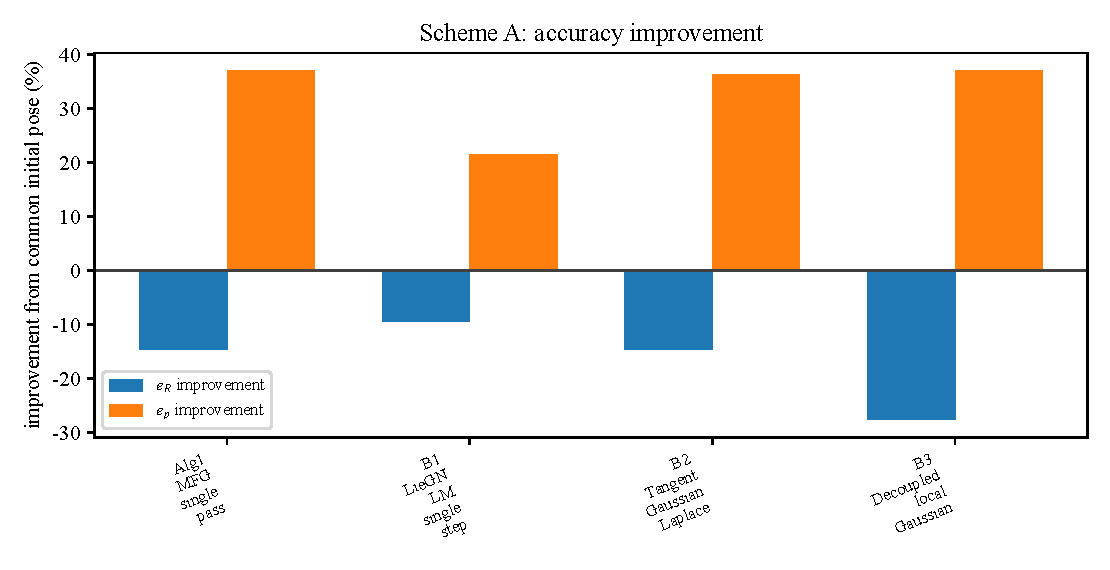
\includegraphics[width=0.48\linewidth]{figures/scheme_A_accuracy_improvement.pdf}\hfill
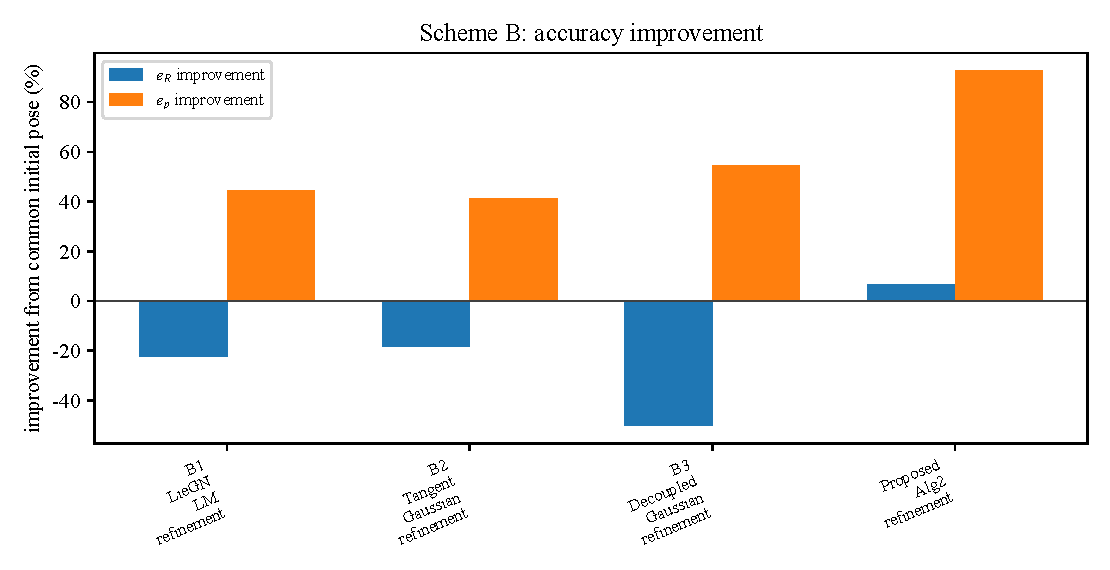
\includegraphics[width=0.48\linewidth]{figures/scheme_B_accuracy_improvement.pdf}
\caption{Mean accuracy improvement from the identical initial pose for
Scheme A and Scheme B.}
\end{figure}

\section*{Reproducibility Notes}
Raw records and summaries are written in \texttt{results/}.  Figures are written
in \texttt{figures/}.  This report was generated with
\texttt{run\_protocol\_accuracy\_baselines.py} using
\texttt{--seeds 42 43 44 45 46 --max-iter 1 --T-max 20}.  All entries
correspond to the same false-confidence Experiment~2C protocol and sparse
measurement design.

\begin{thebibliography}{9}
\bibitem{Levenberg1944}
K. Levenberg, ``A method for the solution of certain non-linear problems in
least squares,'' \emph{Quarterly of Applied Mathematics}, vol. 2, no. 2,
pp. 164--168, 1944.

\bibitem{Marquardt1963}
D. W. Marquardt, ``An algorithm for least-squares estimation of nonlinear
parameters,'' \emph{SIAM Journal on Applied Mathematics}, vol. 11, no. 2,
pp. 431--441, 1963.

\bibitem{NocedalWright2006}
J. Nocedal and S. J. Wright, \emph{Numerical Optimization}, 2nd ed. New York,
NY, USA: Springer, 2006.

\bibitem{Barfoot2017}
T. D. Barfoot, \emph{State Estimation for Robotics}. Cambridge, U.K.:
Cambridge University Press, 2017.

\bibitem{TierneyKadane1986}
L. Tierney and J. B. Kadane, ``Accurate approximations for posterior moments
and marginal densities,'' \emph{Journal of the American Statistical
Association}, vol. 81, no. 393, pp. 82--86, 1986.
\end{thebibliography}

\end{document}
